\section{平面图形分析}
秦奋一脸疑惑的问道:为什么要进行平面图形分析呢?

爸爸:平面图形分析是制图和三维建模工作中一个非常重要且很关键的步骤,是准确绘制图样和构建构模型的基础。平面图形分析的目的是了解平面图形中各图形要素之间相互位置关系,图形之间的依赖关系。图样中的各种尺寸则是用于确定组成图样若干封线框的形状和位置。平面图分析是否准确、是否透彻,直接决定着绘图过程是否正确,也决定着能不能绘制图样和构建模型。

秦奋:平面图形分析主要分析哪些内容?

爸爸:平面图形分析主要是进行平面图形的尺寸分析和平面图形要素的性质分析两个方面的内容。用几张图解释这些内容。

\subsection{平面图形的尺寸分析}
平面图形的尺寸分析的目的主要是确定图形元素的尺寸基准、定形尺寸和定位尺寸三大要素。

\begin{figure}[htbp]
\centering
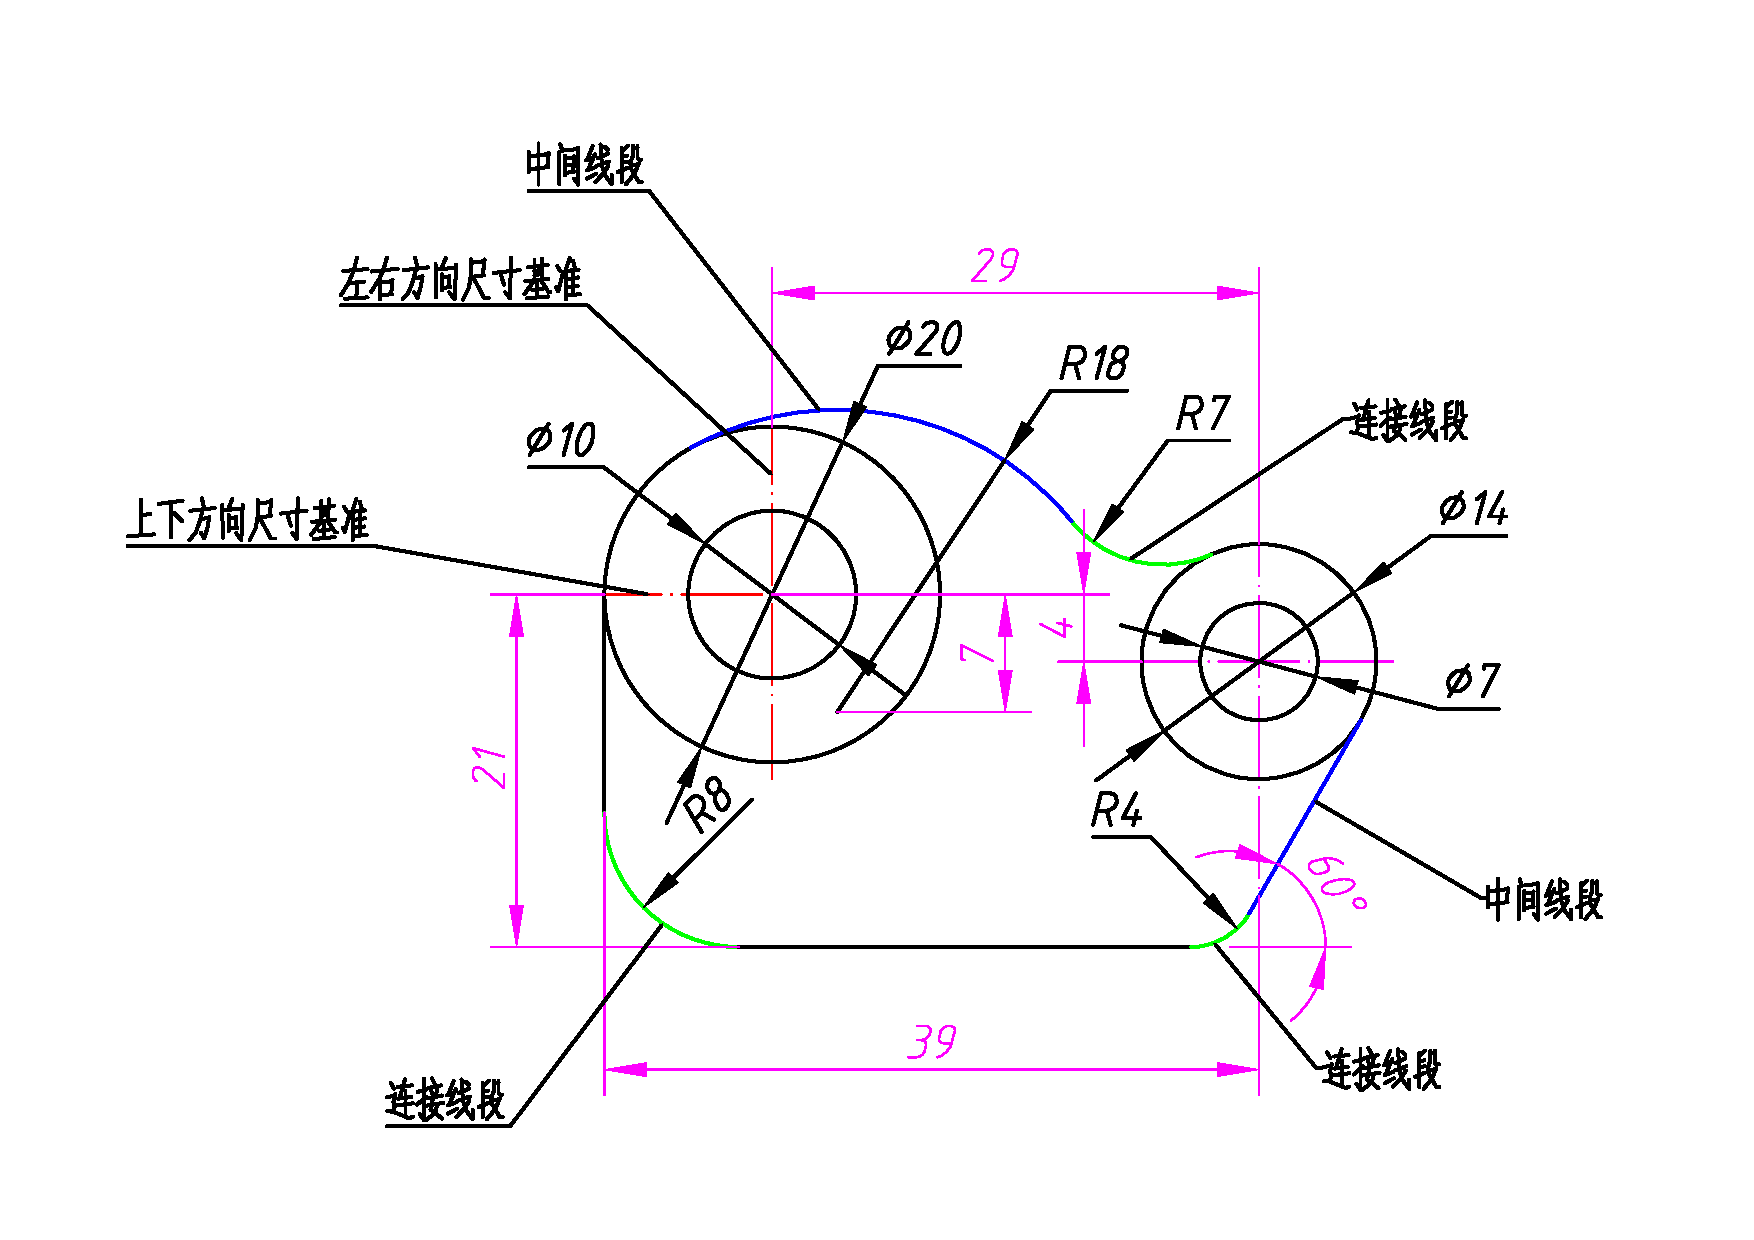
\includegraphics[scale=0.35]{biaozu.pdf}
\caption{平面图形的尺寸和线段分析} \label{fig:biaozu}
\end{figure}

\subsubsection{尺寸基准} 

尺寸基准是绘制和标注尺寸的起点,通常有水平和垂直两个方向的尺寸基准。在具体的工程图样中常常采用图形的对称中心线,较大圆的中心线或主要轮廓线作为尺寸基准线。图\ref{fig:biaozu}所示的图形主要是以长度为99mm的轮廓线和$\phi 20$圆的中心线作为垂直方向和水平方向的尺寸基准。

\subsubsection{定形尺寸} 

定形尺寸是确定平面图形中各线段形状大小的尺寸,如直线的长度、圆和圆弧的直径或半径、角度的大小等。图\ref{fig:biaozu6}中的$\phi 10$、$\phi 20$、 $\phi 14$、 $R8$、$R18$、$R7$等尺寸均为图\ref{fig:biaozu}的定形尺寸。

\begin{figure}[htbp]
\centering
\begin{floatrow}
\ffigbox{\caption{定形尺寸}\label{fig:biaozu6}}{
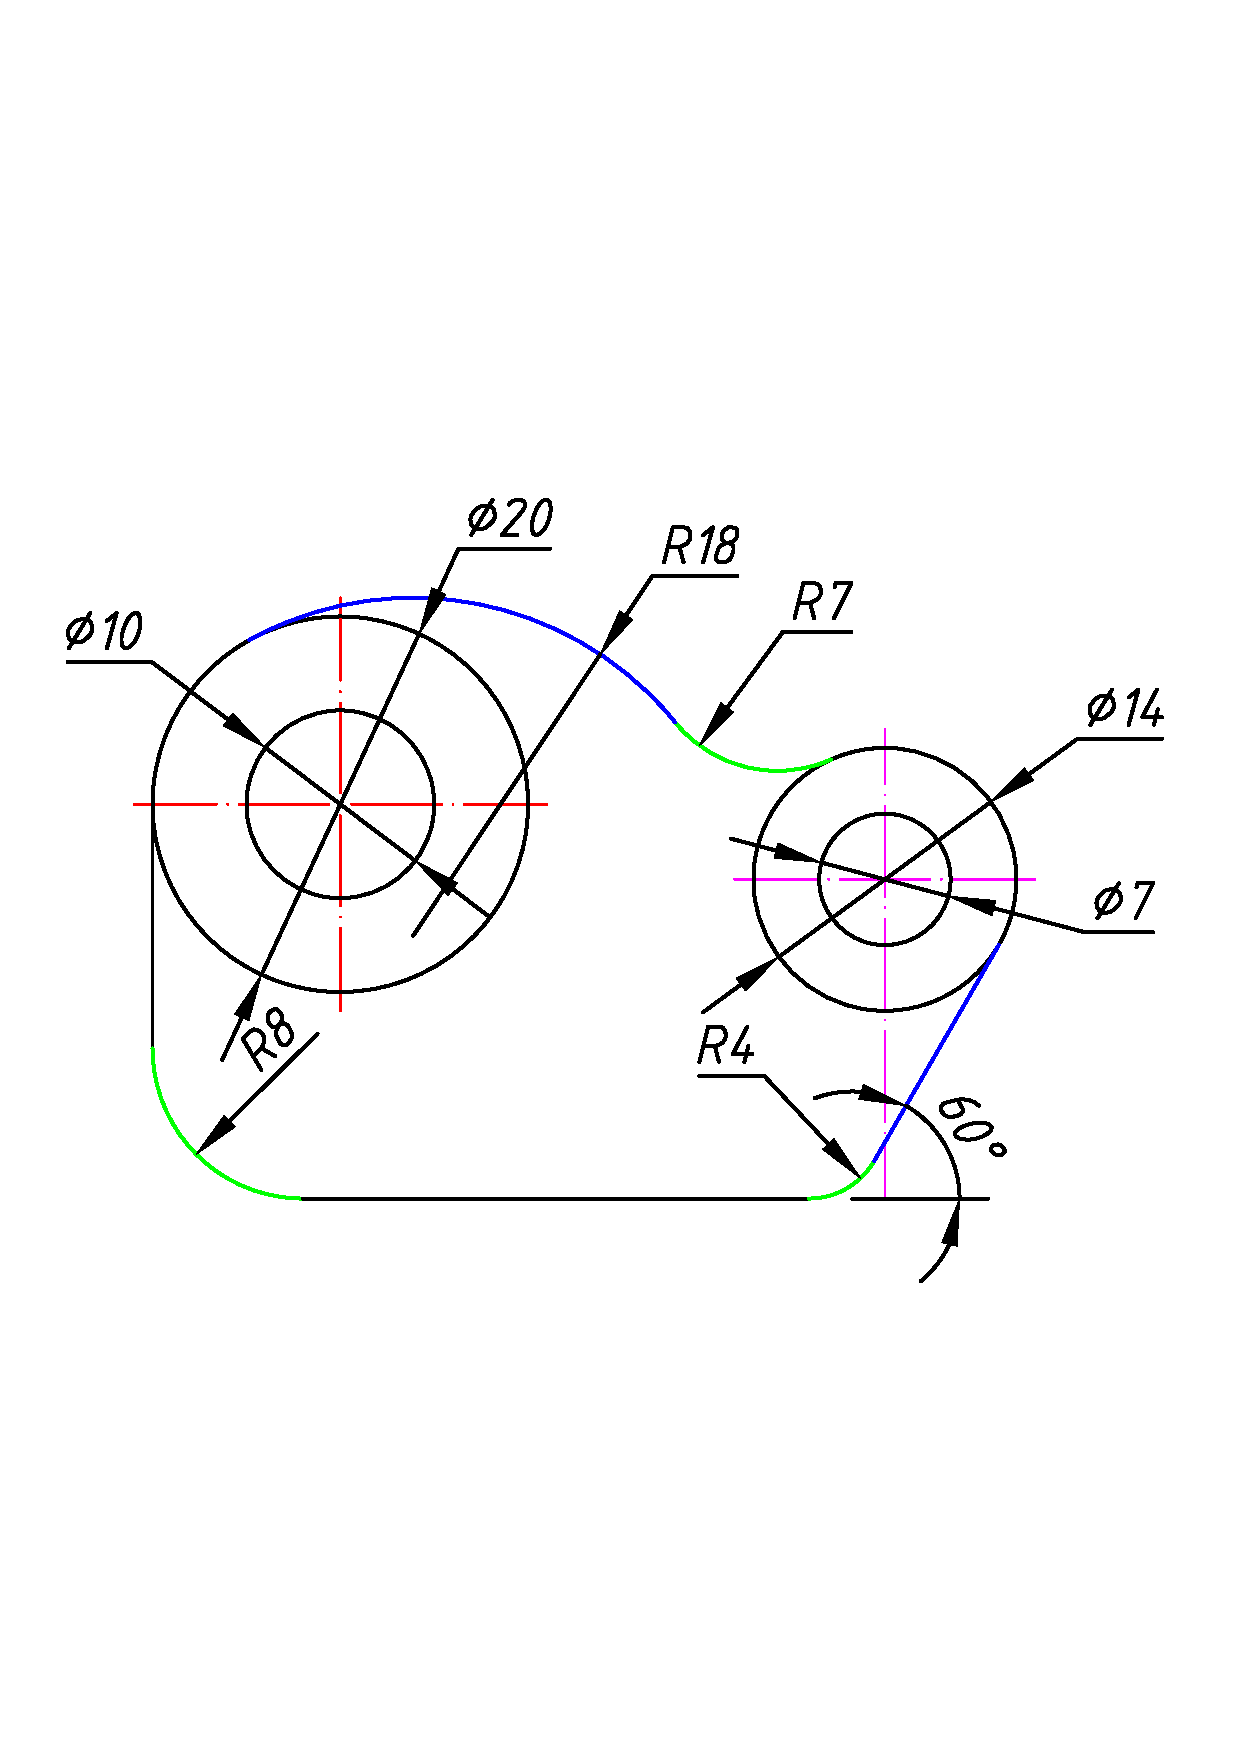
\includegraphics[scale=0.25]{biaozu6.pdf}
}
\ffigbox{\caption{定位尺寸}\label{fig:biaozu5}}{
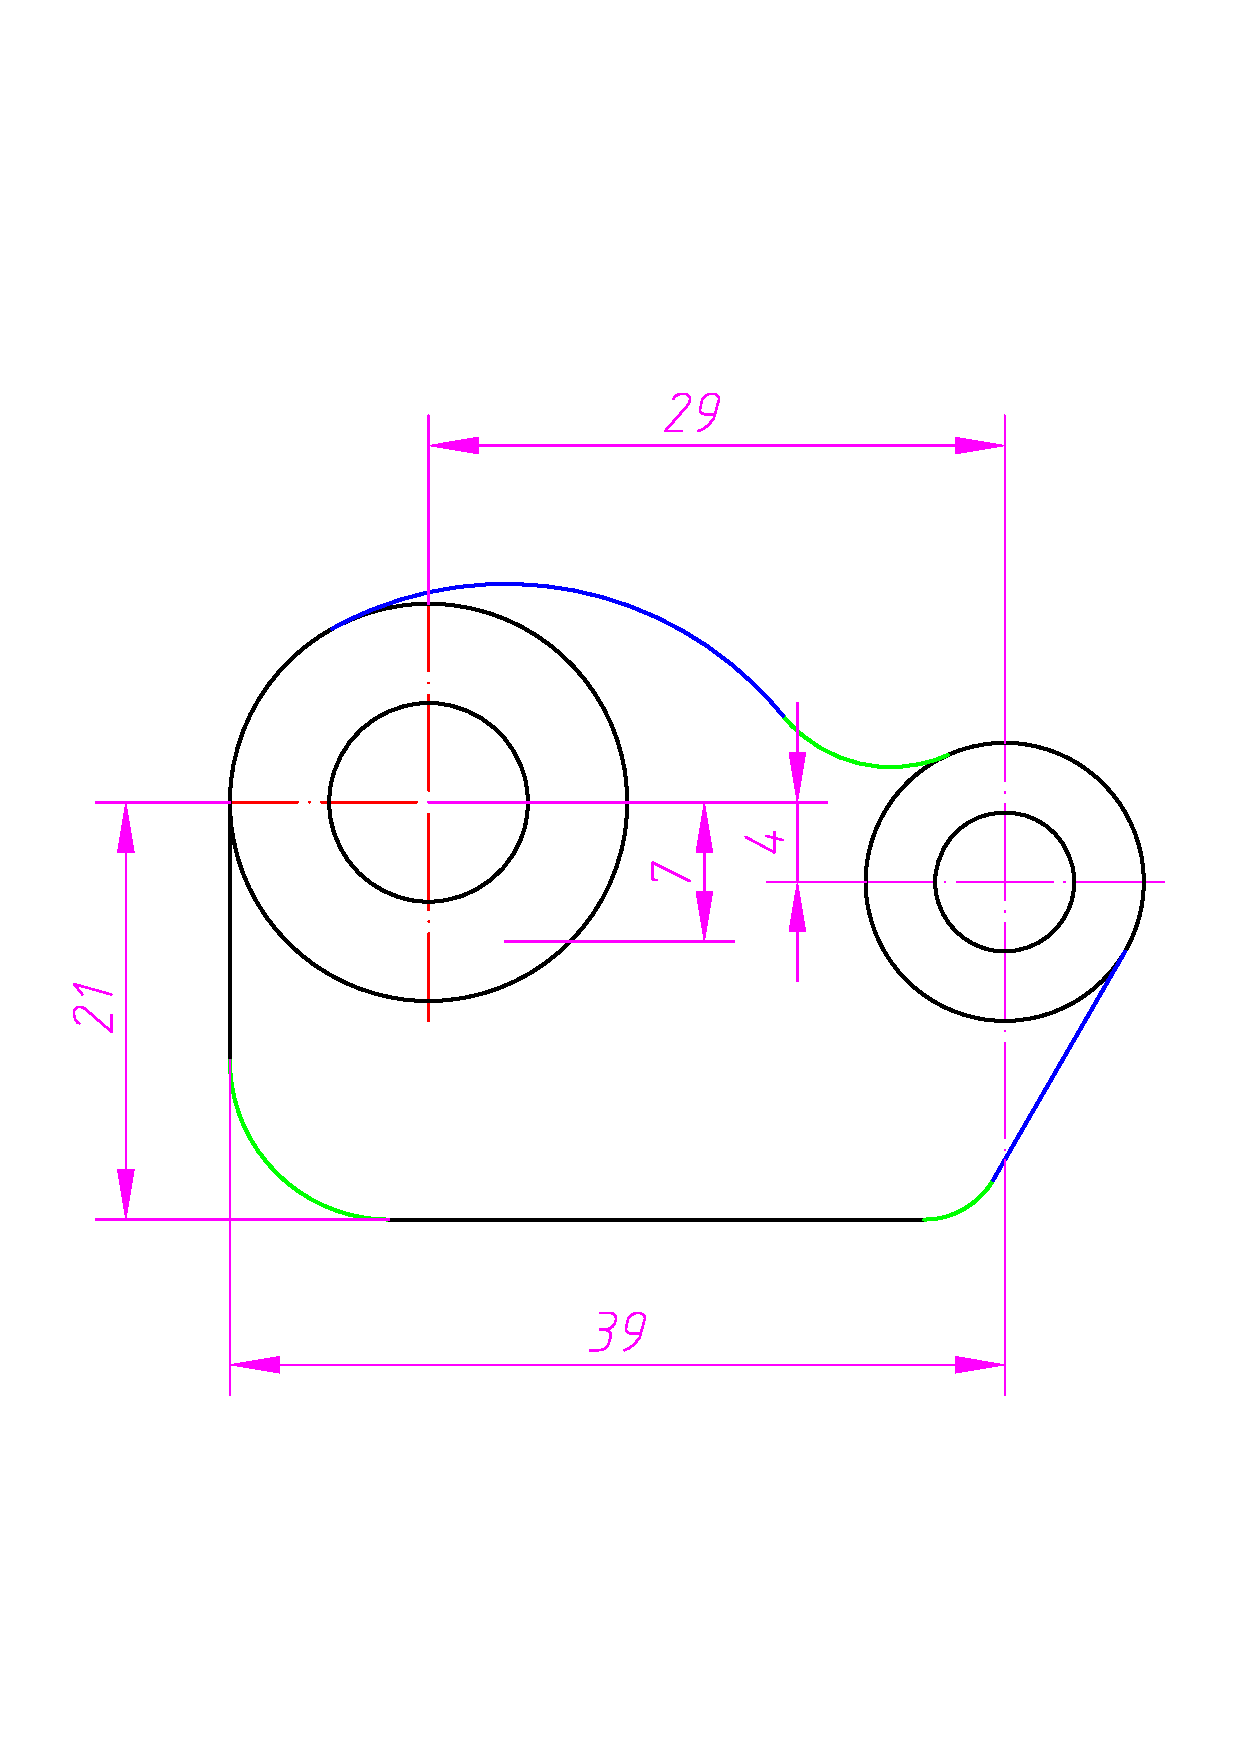
\includegraphics[scale=0.2]{biaozu5.pdf}
}
\end{floatrow}
\end{figure}

\subsubsection{定位尺寸} 

定位尺寸是确定平面图形中各线段之间相对位置的尺寸,图\ref{fig:biaozu5}中标出的尺寸均为图\ref{fig:biaozu}的定位尺寸,其中4和29用于确定$\phi 14$圆的圆心位置。
\endinput